% IPP
% Projekt - 1.
% Juraj Holub
% xholub40@stud.fit.vutbr.cz

\documentclass[a4paper, 10pt]{article}
\usepackage[utf8]{inputenc}
\usepackage[english]{babel}
\usepackage[T1]{fontenc}
\usepackage[left=2cm,top=2.5cm, right=2cm]{geometry}
\usepackage{hyperref}
\usepackage{graphicx}
\usepackage{float}

\title{Documentation of Project Implementation for IPP 2018/2019 }
\author{Name and surname: Juraj Holub\\ Login: xholub40}
\date{}

\begin{document}
	\maketitle
	\thispagestyle{empty}

% proposal of solution
\section{Proposal of solution} \label{proposal}

Solution of interpret program start with parsing source IPPcode19 in XML representation to program inner representation. In this phase program done all necessary syntactic analysys. In next step program interpret parsed IPPcode19 like instructions in right order. In time of interpretation, program done all runtime semantic analyses. Interpret stream output of interpretation to standard output. In case of any syntactic or semantic error, program exit interpretation with specific error return value and generate brief error message to standard error file.
Figure \ref{obr1} shows scheme of implemented interpret program.

\begin{figure}[H] 
	\centering
	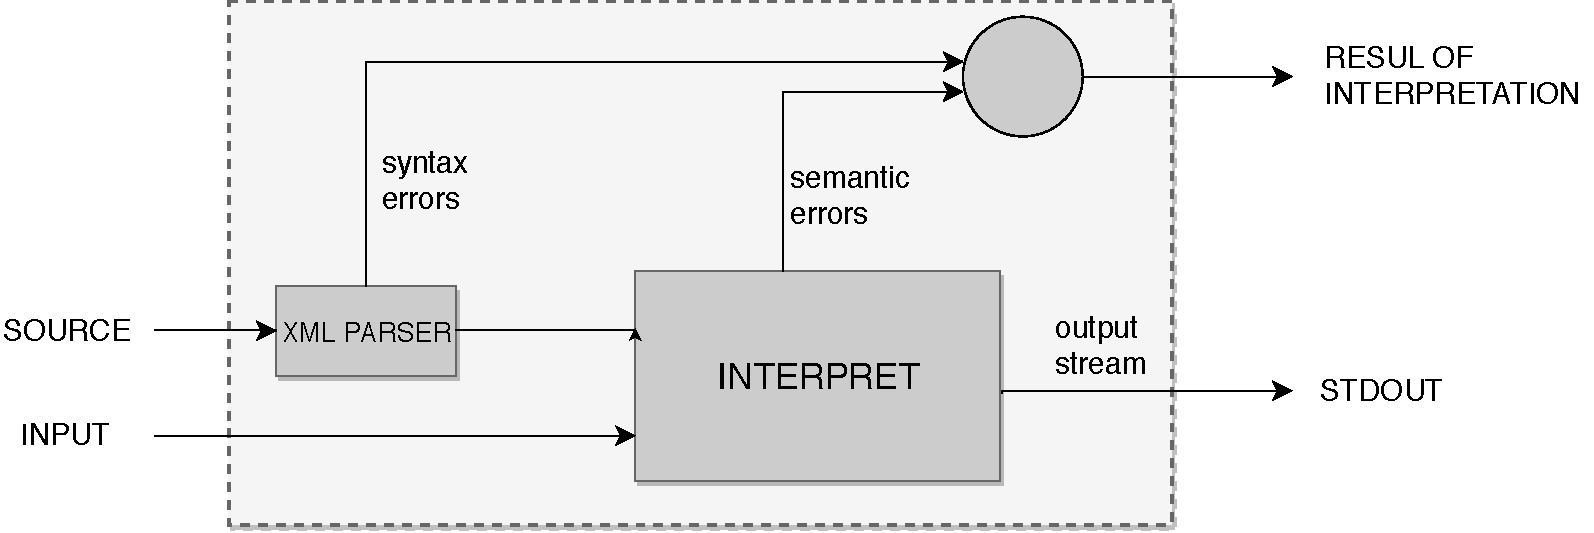
\includegraphics[width=.8 \paperwidth]{interpret.pdf}
	\caption{Scheme of implemented interpretation solution.}
	\label{obr1}
\end{figure} 

\section{Implementation details}
Implementation of solution proposed in section \ref{proposal} is parted to logical blocks described in this section.
\begin{itemize}
	\item \textbf{XML parser}: parse input file to xml, using ElementTree, syntax check, ordering of instruction
	\item \textbf{Interpret}: one method for one instruction, ippcode data are converted to python data representation with equivalent data type (type analyzes could be handled by python it self), in case of runtime error raise exception (described in error handling), program data handling, jumps in program, 
	\item \textbf{Error handling}: syntactic??, semantic handled by catching exception raised in interpret. every runtime error represent one error class, data flushed to stderr about error
	\item \textbf{String convertor}: convert string constant to IPPcode19 string, implemented like FSM
\end{itemize}

\end{document}
